\documentclass[twoside]{book}

% Packages required by doxygen
\usepackage{calc}
\usepackage{doxygen}
\usepackage{graphicx}
\usepackage[utf8]{inputenc}
\usepackage{makeidx}
\usepackage{multicol}
\usepackage{multirow}
\usepackage{fixltx2e}
\PassOptionsToPackage{warn}{textcomp}
\usepackage{textcomp}
\usepackage[nointegrals]{wasysym}
\usepackage[table]{xcolor}

% Font selection
\usepackage[T1]{fontenc}
\usepackage{mathptmx}
\usepackage[scaled=.90]{helvet}
\usepackage{courier}
\usepackage{amssymb}
\usepackage{sectsty}
\renewcommand{\familydefault}{\sfdefault}
\allsectionsfont{%
  \fontseries{bc}\selectfont%
  \color{darkgray}%
}
\renewcommand{\DoxyLabelFont}{%
  \fontseries{bc}\selectfont%
  \color{darkgray}%
}
\newcommand{\+}{\discretionary{\mbox{\scriptsize$\hookleftarrow$}}{}{}}

% Page & text layout
\usepackage{geometry}
\geometry{%
  a4paper,%
  top=2.5cm,%
  bottom=2.5cm,%
  left=2.5cm,%
  right=2.5cm%
}
\tolerance=750
\hfuzz=15pt
\hbadness=750
\setlength{\emergencystretch}{15pt}
\setlength{\parindent}{0cm}
\setlength{\parskip}{0.2cm}
\makeatletter
\renewcommand{\paragraph}{%
  \@startsection{paragraph}{4}{0ex}{-1.0ex}{1.0ex}{%
    \normalfont\normalsize\bfseries\SS@parafont%
  }%
}
\renewcommand{\subparagraph}{%
  \@startsection{subparagraph}{5}{0ex}{-1.0ex}{1.0ex}{%
    \normalfont\normalsize\bfseries\SS@subparafont%
  }%
}
\makeatother

% Headers & footers
\usepackage{fancyhdr}
\pagestyle{fancyplain}
\fancyhead[LE]{\fancyplain{}{\bfseries\thepage}}
\fancyhead[CE]{\fancyplain{}{}}
\fancyhead[RE]{\fancyplain{}{\bfseries\leftmark}}
\fancyhead[LO]{\fancyplain{}{\bfseries\rightmark}}
\fancyhead[CO]{\fancyplain{}{}}
\fancyhead[RO]{\fancyplain{}{\bfseries\thepage}}
\fancyfoot[LE]{\fancyplain{}{}}
\fancyfoot[CE]{\fancyplain{}{}}
\fancyfoot[RE]{\fancyplain{}{\bfseries\scriptsize Generated on Fri May 23 2014 17\+:07\+:03 for Alpha by Doxygen }}
\fancyfoot[LO]{\fancyplain{}{\bfseries\scriptsize Generated on Fri May 23 2014 17\+:07\+:03 for Alpha by Doxygen }}
\fancyfoot[CO]{\fancyplain{}{}}
\fancyfoot[RO]{\fancyplain{}{}}
\renewcommand{\footrulewidth}{0.4pt}
\renewcommand{\chaptermark}[1]{%
  \markboth{#1}{}%
}
\renewcommand{\sectionmark}[1]{%
  \markright{\thesection\ #1}%
}

% Indices & bibliography
\usepackage{natbib}
\usepackage[titles]{tocloft}
\setcounter{tocdepth}{3}
\setcounter{secnumdepth}{5}
\makeindex

% Hyperlinks (required, but should be loaded last)
\usepackage{ifpdf}
\ifpdf
  \usepackage[pdftex,pagebackref=true]{hyperref}
\else
  \usepackage[ps2pdf,pagebackref=true]{hyperref}
\fi
\hypersetup{%
  colorlinks=true,%
  linkcolor=blue,%
  citecolor=blue,%
  unicode%
}

% Custom commands
\newcommand{\clearemptydoublepage}{%
  \newpage{\pagestyle{empty}\cleardoublepage}%
}


%===== C O N T E N T S =====

\begin{document}

% Titlepage & ToC
\hypersetup{pageanchor=false,
             bookmarks=true,
             bookmarksnumbered=true,
             pdfencoding=unicode
            }
\pagenumbering{roman}
\begin{titlepage}
\vspace*{7cm}
\begin{center}%
{\Large Alpha }\\
\vspace*{1cm}
{\large Generated by Doxygen 1.8.7}\\
\vspace*{0.5cm}
{\small Fri May 23 2014 17:07:03}\\
\end{center}
\end{titlepage}
\clearemptydoublepage
\tableofcontents
\clearemptydoublepage
\pagenumbering{arabic}
\hypersetup{pageanchor=true}

%--- Begin generated contents ---
\chapter{Class Index}
\section{Class List}
Here are the classes, structs, unions and interfaces with brief descriptions\+:\begin{DoxyCompactList}
\item\contentsline{section}{\hyperlink{class_conv_layer}{Conv\+Layer} }{\pageref{class_conv_layer}}{}
\end{DoxyCompactList}

\chapter{File Index}
\section{File List}
Here is a list of all documented files with brief descriptions\+:\begin{DoxyCompactList}
\item\contentsline{section}{/\+Users/chengtai/\+Documents/2014/\+M\+O\+T\+R/modules/\+Alpha/\+Alpha/{\bfseries configuration.\+h} }{\pageref{configuration_8h}}{}
\item\contentsline{section}{/\+Users/chengtai/\+Documents/2014/\+M\+O\+T\+R/modules/\+Alpha/\+Alpha/{\bfseries convnet.\+h} }{\pageref{convnet_8h}}{}
\item\contentsline{section}{/\+Users/chengtai/\+Documents/2014/\+M\+O\+T\+R/modules/\+Alpha/\+Alpha/{\bfseries helper.\+h} }{\pageref{helper_8h}}{}
\item\contentsline{section}{/\+Users/chengtai/\+Documents/2014/\+M\+O\+T\+R/modules/\+Alpha/\+Alpha/\hyperlink{layer_8h}{layer.\+h} }{\pageref{layer_8h}}{}
\item\contentsline{section}{/\+Users/chengtai/\+Documents/2014/\+M\+O\+T\+R/modules/\+Alpha/\+Alpha/{\bfseries test.\+h} }{\pageref{test_8h}}{}
\item\contentsline{section}{/\+Users/chengtai/\+Documents/2014/\+M\+O\+T\+R/modules/\+Alpha/\+Alpha/{\bfseries utils.\+h} }{\pageref{utils_8h}}{}
\item\contentsline{section}{/\+Users/chengtai/\+Documents/2014/\+M\+O\+T\+R/modules/\+Alpha/\+Alpha/{\bfseries visual.\+h} }{\pageref{visual_8h}}{}
\end{DoxyCompactList}

\chapter{Class Documentation}
\hypertarget{class_conv_layer}{\section{Conv\+Layer Class Reference}
\label{class_conv_layer}\index{Conv\+Layer@{Conv\+Layer}}
}
Inheritance diagram for Conv\+Layer\+:\begin{figure}[H]
\begin{center}
\leavevmode
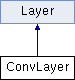
\includegraphics[height=2.000000cm]{class_conv_layer}
\end{center}
\end{figure}
\subsection*{Public Member Functions}
\begin{DoxyCompactItemize}
\item 
\hyperlink{class_conv_layer_a7516441d146b575d8ba191278fe8ba9d}{Conv\+Layer} (int \+\_\+ninmaps, int \+\_\+inputrows, int \+\_\+inputcols, int \+\_\+noutmaps, int \+\_\+stride, int \+\_\+side, int \+\_\+kernelsize, vector$<$ Mat\+Type $>$ $\ast$\+\_\+indata=N\+U\+L\+L)
\item 
\hypertarget{class_conv_layer_ad7b04710a903116d88fcc017b2ca4f2f}{void {\bfseries Set\+Filter} (const vector$<$ vector$<$ Filter\+Type $>$ $>$ \&)}\label{class_conv_layer_ad7b04710a903116d88fcc017b2ca4f2f}

\item 
\hypertarget{class_conv_layer_a585102c25508332b6ab2799409393204}{void {\bfseries Set\+Input} (vector$<$ Mat\+Type $>$ $\ast$)}\label{class_conv_layer_a585102c25508332b6ab2799409393204}

\item 
\hypertarget{class_conv_layer_a8bb67f36834497242e12d0eea4ece95a}{void {\bfseries Set\+Inmaps} (const vector$<$ set$<$ int $>$ $>$ \&)}\label{class_conv_layer_a8bb67f36834497242e12d0eea4ece95a}

\item 
\hypertarget{class_conv_layer_a70111098046a07416fcbdffdbe8f0cfd}{void \hyperlink{class_conv_layer_a70111098046a07416fcbdffdbe8f0cfd}{Apply\+Filter} ()}\label{class_conv_layer_a70111098046a07416fcbdffdbe8f0cfd}

\begin{DoxyCompactList}\small\item\em T\+O\+D\+O\+: the index order is filter\mbox{[}j\mbox{]}\mbox{[}i\mbox{]}, inmaps\mbox{[}j\mbox{]}\mbox{[}i\mbox{]}, not the other way around. \end{DoxyCompactList}\item 
\hypertarget{class_conv_layer_a8970249425ba935d91bc0f0a530ea13c}{void {\bfseries Down\+Sample} ()}\label{class_conv_layer_a8970249425ba935d91bc0f0a530ea13c}

\item 
\hypertarget{class_conv_layer_a5e5a5da58cb21ca2894ecf55088a2636}{void {\bfseries Apply\+Nonlinearity} ()}\label{class_conv_layer_a5e5a5da58cb21ca2894ecf55088a2636}

\item 
\hypertarget{class_conv_layer_aea08727ba47d3c813e309cc278860bbd}{bool {\bfseries Self\+Check} ()}\label{class_conv_layer_aea08727ba47d3c813e309cc278860bbd}

\end{DoxyCompactItemize}
\subsection*{Public Attributes}
\begin{DoxyCompactItemize}
\item 
\hypertarget{class_conv_layer_a3fbf8929ebf39d70281c548653159fe1}{vector$<$ vector$<$ Filter\+Type $>$ $>$ {\bfseries filter}}\label{class_conv_layer_a3fbf8929ebf39d70281c548653159fe1}

\item 
\hypertarget{class_conv_layer_ae90ccdaf98509ac518dc8158abb53540}{vector$<$ Mat\+Type $>$ $\ast$ {\bfseries indata}}\label{class_conv_layer_ae90ccdaf98509ac518dc8158abb53540}

\item 
\hypertarget{class_conv_layer_a41e52948623d345d93ddf7e3e6d4098c}{vector$<$ Mat\+Type $>$ {\bfseries outdata}}\label{class_conv_layer_a41e52948623d345d93ddf7e3e6d4098c}

\item 
\hypertarget{class_conv_layer_a2a829e399b291ef09856b71484ddcade}{vector$<$ set$<$ int $>$ $>$ {\bfseries inmaps}}\label{class_conv_layer_a2a829e399b291ef09856b71484ddcade}

\item 
\hypertarget{class_conv_layer_a9c41797df74c1eef60fb4fdbf2713379}{string {\bfseries name}}\label{class_conv_layer_a9c41797df74c1eef60fb4fdbf2713379}

\item 
\hypertarget{class_conv_layer_a62ef7802fa2cb90f2a6c3f09f52d1485}{const int {\bfseries ninmaps}}\label{class_conv_layer_a62ef7802fa2cb90f2a6c3f09f52d1485}

\item 
\hypertarget{class_conv_layer_a24e3feabcb086d6a9985c263b954f32e}{const int {\bfseries inputrows}}\label{class_conv_layer_a24e3feabcb086d6a9985c263b954f32e}

\item 
\hypertarget{class_conv_layer_a51c24316490e75baea4950781a65d7f9}{const int {\bfseries inputcols}}\label{class_conv_layer_a51c24316490e75baea4950781a65d7f9}

\item 
\hypertarget{class_conv_layer_a5b16865e198761926c2f4820062b0766}{const int {\bfseries noutmaps}}\label{class_conv_layer_a5b16865e198761926c2f4820062b0766}

\item 
\hypertarget{class_conv_layer_a503460202a6877759475b94e8bda8aa6}{const int {\bfseries stride}}\label{class_conv_layer_a503460202a6877759475b94e8bda8aa6}

\item 
\hypertarget{class_conv_layer_aa393a1694d13a8d62f3eddc1709e5b74}{const int {\bfseries side}}\label{class_conv_layer_aa393a1694d13a8d62f3eddc1709e5b74}

\item 
\hypertarget{class_conv_layer_ad0f8a1eab56d2db1309913de2b299fc9}{const int {\bfseries kernelsize}}\label{class_conv_layer_ad0f8a1eab56d2db1309913de2b299fc9}

\end{DoxyCompactItemize}


\subsection{Constructor \& Destructor Documentation}
\hypertarget{class_conv_layer_a7516441d146b575d8ba191278fe8ba9d}{\index{Conv\+Layer@{Conv\+Layer}!Conv\+Layer@{Conv\+Layer}}
\index{Conv\+Layer@{Conv\+Layer}!Conv\+Layer@{Conv\+Layer}}
\subsubsection[{Conv\+Layer}]{\setlength{\rightskip}{0pt plus 5cm}Conv\+Layer\+::\+Conv\+Layer (
\begin{DoxyParamCaption}
\item[{int}]{\+\_\+ninmaps, }
\item[{int}]{\+\_\+inputrows, }
\item[{int}]{\+\_\+inputcols, }
\item[{int}]{\+\_\+noutmaps, }
\item[{int}]{\+\_\+stride, }
\item[{int}]{\+\_\+side, }
\item[{int}]{\+\_\+kernelsize, }
\item[{vector$<$ Mat\+Type $>$ $\ast$}]{\+\_\+indata = {\ttfamily NULL}}
\end{DoxyParamCaption}
)\hspace{0.3cm}{\ttfamily [inline]}}}\label{class_conv_layer_a7516441d146b575d8ba191278fe8ba9d}

\begin{DoxyParams}{Parameters}
{\em \+\_\+ninmaps} & Number of input maps. \\
\hline
{\em \+\_\+inputrows} & Number of rows of input matrix. \\
\hline
{\em \+\_\+inputcols} & Number of columns of input matrix. \\
\hline
{\em \+\_\+noutmaps} & Number of maps of this layer. \\
\hline
{\em \+\_\+stride} & stride. \\
\hline
{\em \+\_\+side} & side. \\
\hline
{\em \+\_\+kernelsize} & kernelsize, must be square. \\
\hline
{\em \+\_\+indata.} & Input data, optional. \\
\hline
\end{DoxyParams}


The documentation for this class was generated from the following files\+:\begin{DoxyCompactItemize}
\item 
/\+Users/chengtai/\+Documents/2014/\+M\+O\+T\+R/modules/\+Alpha/\+Alpha/\hyperlink{layer_8h}{layer.\+h}\item 
/\+Users/chengtai/\+Documents/2014/\+M\+O\+T\+R/modules/\+Alpha/\+Alpha/layer.\+cpp\end{DoxyCompactItemize}

\chapter{File Documentation}
\hypertarget{helper_8h}{\section{/\+Users/chengtai/\+Documents/2014/\+M\+O\+T\+R/modules/\+Alpha/\+Alpha/helper.h File Reference}
\label{helper_8h}\index{/\+Users/chengtai/\+Documents/2014/\+M\+O\+T\+R/modules/\+Alpha/\+Alpha/helper.\+h@{/\+Users/chengtai/\+Documents/2014/\+M\+O\+T\+R/modules/\+Alpha/\+Alpha/helper.\+h}}
}


This is a test.  


\subsection*{Functions}
\begin{DoxyCompactItemize}
\item 
\hypertarget{helper_8h_a06737a71a82b746a220d3c6a6bade850}{void \hyperlink{helper_8h_a06737a71a82b746a220d3c6a6bade850}{Load\+Filter} (vector$<$ Filter\+Type $>$ \&filter, string fname)}\label{helper_8h_a06737a71a82b746a220d3c6a6bade850}

\begin{DoxyCompactList}\small\item\em Available test. \end{DoxyCompactList}\item 
\hypertarget{helper_8h_a66288b9b809be113d49ee7a03fa40e5c}{Mat\+Type {\bfseries Conv2\+\_\+\+Valid} (const Mat\+Type \&a, const Mat\+Type \&b)}\label{helper_8h_a66288b9b809be113d49ee7a03fa40e5c}

\item 
\hypertarget{helper_8h_a478da42f4930ff868d028cb0e5b6bebf}{Mat\+Type {\bfseries Conv2} (const Mat\+Type \&a, const Mat\+Type \&b, Boundary\+Type boundarytype)}\label{helper_8h_a478da42f4930ff868d028cb0e5b6bebf}

\end{DoxyCompactItemize}


\subsection{Detailed Description}
This is a test. 


%--- End generated contents ---

% Index
\newpage
\phantomsection
\addcontentsline{toc}{chapter}{Index}
\printindex

\end{document}
